\documentclass{article}
\usepackage[utf8]{inputenc}
\usepackage[margin=1.0in]{geometry}
\usepackage{amsmath}
\usepackage{amssymb}
\usepackage{fancyhdr}
\usepackage{physics}
\usepackage{wrapfig}
\usepackage{hyperref}
\usepackage{multirow}
\usepackage{amsthm}
\usepackage{float}
\usepackage{pgfplots}

\pgfplotsset{compat=1.16}



\renewcommand{\thesubsection}{\thesection\Alph{subsection}}
\renewcommand\qedsymbol{\square}



\title{Quantum Mechanics PS3}
\author{Joe Crowley}
\date{October 2020}

\pagestyle{fancy}
\renewcommand{\headrulewidth}{0pt}
\renewcommand{\footrulewidth}{1pt}

\fancyhf{}
\rhead{
Joe Crowley \\
Physics 215 \\
Problem Set 2\\
}
\rfoot{Page \thepage}

\begin{document}  

\section{SN 1.2}
\textit{Suppose a $2 \times 2$ matrix $X$ (not necessarily Hermitian or unitary) is written as
$$
X=a_{0}+\vec{\sigma} \cdot \vec{a}
$$
where $a_{0}$ and $a_{1,2,3}$ are numbers.}
\subsection{}
\textit{How are $a_{0}$ and $a_{k}(k=1,2,3)$ related to $\mathbf{tr}(X)$ and $\mathbf{tr}\left(\sigma_{k} X\right) ?$}
\begin{align*}
    X&=a_{0}+\vec{\sigma} \cdot \vec{a}\\
    &=a_{0}+\left(\begin{array}{ll}
0 & 1 \\
1 & 0
\end{array}\right) a_{1}+\left(\begin{array}{cc}
0 & -i \\
i & 0
\end{array}\right) a_{2}+\left(\begin{array}{cc}
1 & 0 \\
0 & -1
\end{array}\right) a_{3}\\
\end{align*}

\begin{equation*}
     \mathbf{Tr}(X)=a_{0} \mathbf{Tr}(1)=2 a_{0}
\end{equation*}

\begin{equation*}
    \sigma_{k} X=a_{0} \sigma_{k}+\sigma_{k} \vec{\sigma} \cdot \vec{a}
\end{equation*}


\begin{align*}
    \mathbf{Tr}\left(\sigma_{k} X\right)&=a_{0} \mathbf{Tr}\left(\sigma_{k}\right)+\sum_{\ell} \mathbf{Tr}\left(\sigma_{k} \sigma_{\ell} a_{\ell}\right)\\
    &=a_{0} \mathbf{Tr}\left(\sigma_{k}\right)+\frac{1}{2} \sum_{\ell} \mathbf{Tr}\left(\sigma_{k} \sigma_{\ell}+\sigma_{\ell} \sigma_{k}\right) a_{\ell}\\
    &=\sum_{\ell} \delta_{k \ell} \mathbf{Tr}(1) a_{\ell}\\
    &= 2 a_{k}
\end{align*}


\begin{equation*}
    \boxed{\begin{align*}
            a_{0}&=\frac{1}{2}\mathbf{Tr}(X)\\
            a_{k}&=\frac{1}{2} \mathbf{Tr}\left(\sigma_{k} X\right)\\
        \end{align*}}
\end{equation*}


\subsection{}
\textit{Obtain $a_{0}$ and $a_{k}$ in terms of the matrix elements $X_{i j}$}


\begin{align*}
    a_{0}&=\frac{1}{2}\mathbf{Tr}(X) = \frac{1}{2}(X_{11} + X_{22})\\
    a_{1}&=\frac{1}{2} \mathbf{Tr}\left(\sigma_{1} X\right) = \frac{1}{2}(X_{12} + X_{21})\\
    a_{2}&=\frac{1}{2} \mathbf{Tr}\left(\sigma_{2} X\right) = \frac{i}{2}(X_{12} - X_{21})\\
    a_{3}&=\frac{1}{2} \mathbf{Tr}\left(\sigma_{3} X\right) = \frac{1}{2}(X_{11} - X_{22})\\
\end{align*}

\newpage

\section{SN 1.8}
\textit{Using the orthonormality of $\ket{0}$ and $\ket{1},$ prove
$$
\left[S_{i}, S_{j}\right]=i \varepsilon_{i j k} \hbar S_{k}, \quad\left\{S_{i}, S_{j}\right\}=\left(\frac{\hbar^{2}}{2}\right) \delta_{i j}
$$
where
$$
\begin{array}{l}
S_{x}=\frac{\hbar}{2}(\ketbra{0}{1}+\ketbra{1}{0}), \quad S_{y}=\frac{i \hbar}{2}(-\ketbra{0}{1}+\ketbra{1}{0}) \\
S_{z}=\frac{\hbar}{2}(\ketbra{0}{0}-\ketbra{1}{1})
\end{array}
$$}

\begin{align*}
    [\hat{S}_x, \hat{S}_y] &= \frac{i \hbar^2 }{4}\left[(\ketbra{0}{1}+\ketbra{1}{0})(-\ketbra{0}{1}+\ketbra{1}{0}) - (-\ketbra{0}{1}+\ketbra{1}{0})(\ketbra{0}{1}+\ketbra{1}{0})\right]\\
    &= \frac{i \hbar^2 }{4} (-2\ketbra{1}{1} +  2 \ketbra{0}{0} )\\
    &= \frac{i \hbar^2 }{2} (-\ketbra{1}{1} +   \ketbra{0}{0} )\\
    &= i \hbar \hat{S}_z 
\end{align*}


\begin{align*}
    [\hat{S}_y, \hat{S}_z] &= \frac{i \hbar^2 }{4}\left[(-\ketbra{0}{1}+\ketbra{1}{0})(\ketbra{0}{0}-\ketbra{1}{1}) - (\ketbra{0}{0}-\ketbra{1}{1})(-\ketbra{0}{1}+\ketbra{1}{0})\right]\\
    &= \frac{i \hbar^2 }{4} (2\ketbra{0}{1}+2\ketbra{1}{0}) )\\
    &= i \hbar \hat{S}_x 
\end{align*}

\begin{align*}
    [\hat{S}_z, \hat{S}_x] &= \frac{i \hbar^2 }{4}\left[(\ketbra{0}{0}-\ketbra{1}{1})(\ketbra{0}{1}+\ketbra{1}{0}) - (\ketbra{0}{1}+\ketbra{1}{0})(\ketbra{0}{0}-\ketbra{1}{1})\right]\\
    &= \frac{i \hbar^2 }{4}(-2\ketbra{0}{1}+2\ketbra{1}{0}))\\
    &= i \hbar \hat{S}_y 
\end{align*}

\begin{align*}
    \{\hat{S}_x, \hat{S}_y\} &= \frac{i \hbar^2 }{4}\left[(\ketbra{0}{1}+\ketbra{1}{0})(-\ketbra{0}{1}+\ketbra{1}{0}) + (-\ketbra{0}{1}+\ketbra{1}{0})(\ketbra{0}{1}+\ketbra{1}{0})\right]\\
    &= \frac{i \hbar^2 }{4} (2\ketbra{1}{1} +  2 \ketbra{0}{0} )\\
    &= \frac{i \hbar^2 }{2} (\ketbra{1}{1} +   \ketbra{0}{0} )\\
    &= 0
\end{align*}

\begin{align*}
    \{\hat{S}_x, \hat{S}_x\} &= \frac{ \hbar^2 }{4}\left[(\ketbra{0}{1}+\ketbra{1}{0})(\ketbra{0}{1}+\ketbra{1}{0}) + (\ketbra{0}{1}+\ketbra{1}{0})(\ketbra{0}{1}+\ketbra{1}{0})\right]\\
    &= \frac{ \hbar^2 }{4} (2\ketbra{1}{1} +  2 \ketbra{0}{0} )\\
    &= \frac{ \hbar^2 }{2} (\ketbra{1}{1} +   \ketbra{0}{0} )\\
    &=  \frac{ \hbar^2 }{2} \hat 1
\end{align*}




\newpage

\section{SN 1.9}
\textit{Construct $\ket{\hat{\mathbf{S}} \cdot \hat{\mathbf{n}} ;+}$ such that
$$
\hat{\mathbf{S}} \cdot \hat{\mathbf{n}}\ket{\hat{\mathbf{S}} \cdot \hat{\mathbf{n}} ;0}=\left(\frac{\hbar}{2}\right)\ket{\hat{\mathbf{S}} \cdot \hat{\mathbf{n}} ;0}
$$
where $\hat{\mathbf{n}}$ is characterized by the angles shown in the accompanying figure. Express your answer as a linear combination of $\ket{0}$ and $\ket{1} .[$Note: The answer is
$$
\cos \left(\frac{\beta}{2}\right)\ket{0}+\sin \left(\frac{\beta}{2}\right) e^{i \alpha}\ket{1}
$$
But do not just verify that this answer satisfies the above eigenvalue equation. Rather, treat the problem as a straightforward eigenvalue problem. Also, do not use rotation operators, which we will introduce later in this book.$]$}

\begin{equation*}
    \hat{\mathbf{n}}=\cos \alpha \sin \beta \hat{\mathbf{x}} + \sin \alpha \sin \beta \hat{\mathbf{y}}+ \cos \beta \hat{\mathbf{z}}
\end{equation*}

\begin{align*}
    \hat{\mathbf{S}} \cdot \hat{\mathbf{n}} &= S_{x} \cos \alpha \sin \beta+S_{y} \sin \alpha \sin \beta+S_{z} \cos \beta\\
    &=\left(\begin{array}{cc}
\cos \beta & e^{-i \alpha} \sin \beta \\
e^{i \alpha} \sin \beta & -\cos \beta
\end{array}\right)
\end{align*}

\begin{align*}
    \hat{\mathbf{S}} \cdot \hat{\mathbf{n}}\left(\begin{array}{l}
    a \\
    b
    \end{array}\right)=\left(\begin{array}{l}
    a \\
    b
    \end{array}\right)\\
    \left(\begin{array}{cc}
\cos \beta & e^{-i \alpha} \sin \beta \\
e^{i \alpha} \sin \beta & -\cos \beta
\end{array}\right)\left(\begin{array}{l}
    a \\
    b
    \end{array}\right) = \left(\begin{array}{l}
    a \\
    b
    \end{array}\right)\\
\end{align*}    
\begin{align*}
a \cos \beta+b e^{-i \alpha} \sin \beta &=a \\
a e^{i \alpha} \sin \beta-b \cos \beta &=b
\end{align*}

\begin{align*}
    a&=\cos (\beta / 2)\\
    b&= e^{i \alpha} \sin (\beta / 2) 
\end{align*}

\begin{equation*}
\boxed{
    \ket{\hat{\mathbf{S}} \cdot \hat{\mathbf{n}} ;+} = \cos (\beta / 2) \ket{0} + e^{i \alpha} \sin (\beta / 2) \ket{1}
    }
\end{equation*}


\newpage
\section{SN 1.10}
\textit{The Hamiltonian operator for a two-state system is given by
$$
H=a(\ketbra{1}{1}-\ketbra{2}{2}+\ketbra{1}{2}+\ketbra{2}{1})
$$
where $a$ is a number with the dimension of energy. Find the energy eigenvalues and the corresponding energy eigenkets $($as linear combinations of $\ket{1} and \ket{2}$ $)$.}


\begin{align*}
    \hat{H}&=a\left(\begin{array}{ll}
        1 & 1 \\
        1 & -1
        \end{array}\right)\\
    &= \left(\begin{array}{ll}
        a & a \\
        a & -a
        \end{array}\right)
\end{align*}

\begin{align*}
    \operatorname{det}(\hat{H}-\lambda)&=0\\
    (a-\lambda)(-a-\lambda)-a^{2}&=0\\
    \lambda^{2}&=2 a^{2}
\end{align*}

$$\boxed{\lambda=\pm \sqrt{2} a}$$

\begin{equation*}
        \hat{H} \ket{\psi}=\left(\begin{array}{ll}
        a & a \\
        a & -a
        \end{array}\right)\left(\begin{array}{l}
        \psi_1 \\
        \psi_{2}
        \end{array}\right)
\end{equation*}


\begin{equation*}
        \left(\begin{array}{ll}
        a & a \\
        a & -a
        \end{array}\right)\left(\begin{array}{l}
        \psi_1 \\
        \psi_{2}
        \end{array}\right) = \pm \sqrt{2} a \left(\begin{array}{l}
        \psi_1 \\
        \psi_{2}
        \end{array}\right)
\end{equation*}


\begin{equation*}
    \psi_2 = (\pm \sqrt{2} - 1) \psi_1
\end{equation*}

\begin{equation*}
    \boxed{\ket{\pm \sqrt{2} a} = \frac{1}{\sqrt{1+(\pm \sqrt{2}+1)^{2}}}\left(\begin{array}{c}
1 \\
\pm \sqrt{2}-1
\end{array}\right)}
\end{equation*}




\newpage

\section{SN 1.11}
\textit{A two-state system is characterized by the Hamiltonian
$$
H=H_{11}\ketbra{1}{1}+H_{22}\ketbra{2}{2}+H_{12}[\ketbra{1}{2}+\ketbra{2}{1}]
$$
where $H_{11}, H_{22},$ and $H_{12}$ are real numbers with the dimension of energy, and $\ket{1}$ and $\ket{2}$ are eigenkets of some observable $(\neq H) .$ Find the energy eigenkets and the corresponding energy eigenvalues. Make sure that your answer makes good sense for $H_{12}=0 .$ (You need not solve this problem from scratch. The following fact may be used without proof:
$$
(\mathbf{S} \cdot \hat{\mathbf{n}})\ket{\hat{\mathbf{n}} ;+}=\frac{\hbar}{2}\ket{\hat{\mathbf{n}} ;+}
$$
with $\ket{\hat{\mathbf{n}} ;+}$ given by
$$
\ket{\hat{\mathbf{n}} ;+}=\cos \frac{\beta}{2}\ket{+}+e^{i \alpha} \sin \frac{\beta}{2}\ket{-}
$$
where $\beta$ and $\alpha$ are the polar and azimuthal angles, respectively, that characterize $\hat{\mathbf{n}}$. The angles are defined in the figure following Problem 1.9.)}

\begin{figure}[H]
    \centering
    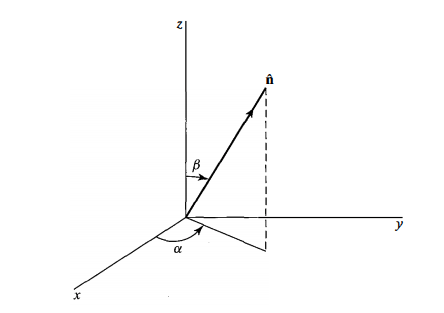
\includegraphics[width=0.4\textwidth]{figures/problem5.png}
    \label{fig:my_label}
\end{figure}


\begin{align*}
0&=\left(H_{11}-\lambda\right)\left(H_{22}-\lambda\right)-H_{12}^{2} \\
&=H_{11} H_{22}-H_{11} \lambda -H_{12}^2-H_{22} \lambda +\lambda ^2\\
\implies \lambda_\pm &= \frac{1}{2}\left(\pm\sqrt{H_{11}^2-2 H_{11} H_{22}+4 H_{12}^2+H_{22}^2}+H_{11}+H_{22}\right)
\end{align*}


\begin{align*}
    \hat{H} \ket{\lambda_\pm} &= \lambda_\pm \ket{\lambda_\pm}\\
    \hat{H} \left(\begin{array}{l}
        a \\
        b
        \end{array}\right) &= \lambda_\pm \left(\begin{array}{l}
        a \\
        b
        \end{array}\right)\\
        \left(\begin{array}{l}
b H_{12}+a H_{11} \\
b H_{22}+a H_{12}
\end{array}\right)&=\left(\begin{array}{c}
\frac{a}{2}\left(\pm \sqrt{H_{11}^{2}-2 H_{11} H_{22}+4 H_{12}^{2}+H_{22}^{2}}+H_{11}+H_{22}\right) \\
\frac{b}{2} \left(\pm \sqrt{H_{11}^{2}-2 H_{11} H_{22}+4 H_{12}^{2}+H_{22}^{2}}+H_{11}+H_{22}\right)
\end{array}\right)\\
&\\
b &= \mp \frac{a \sqrt{H_{11}^2-2 H_{11} H_{22}+4 H_{12}^2+H_{22}^2}+a H_{11}-a H_{22}}{2 H_{12}}
\end{align*}

$$\ket{\lambda_\pm} =  \left(\begin{array}{l}
        1 \\
        \mp \frac{ \sqrt{H_{11}^2-2 H_{11} H_{22}+4 H_{12}^2+H_{22}^2}+ H_{11}- H_{22}}{2 H_{12}}
        \end{array}\right)
$$

\newpage

\section{SN 1.12}
\textit{A spin $\frac{1}{2}$ system is known to be in an eigenstate of $\hat{\mathbf{S}} \cdot \hat{\mathbf{n}}$ with eigenvalue $\hbar / 2,$ where n is a unit vector lying in the $x z$ -plane that makes an angle $\gamma$ with the positive $z$ -axis.}
\subsection{}
\textit{Suppose $S_{x}$ is measured. What is the probability of getting $+\hbar / 2 ?$}
$$\ket{\psi} = \cos (\frac{\gamma }{2}) \ket{0_z} + \sin (\frac{\gamma }{2}) \ket{1_z}$$

$$ \bra{0_x} =  \frac{1}{\sqrt{2}}(\bra{0_z} + \bra{1_z})$$


\begin{align*}
\left|\braket{0_x}{\psi}\right|^2 &= \frac{1}{\sqrt{2}}(\bra{0_z} + \bra{1_z}) \left( \cos (\frac{\gamma }{2}) \ket{0_z} + \sin (\frac{\gamma }{2}) \ket{1_z}\right)\\
&= \left(\frac{\sin \left(\frac{\gamma }{2}\right)}{\sqrt{2}}+\frac{\cos \left(\frac{\gamma }{2}\right)}{\sqrt{2}}\right)^2\\
&= \frac{1}{2}\left(\sqrt{\frac{1-\cos \gamma}{2}}+\sqrt{\frac{1+\cos \gamma}{2}}\right)^{2}\\
&= \frac{1+\sin \gamma}{2}\\
\end{align*}

$$\boxed{\left|\braket{0_x}{\psi}\right|^2= \frac{1+\sin \gamma}{2}}$$

\subsection{}
\textit{Evaluate the dispersion in $S_{x}$, that is,
$$
\left\langle\left(S_{x}-\left\langle S_{x}\right\rangle\right)^{2}\right\rangle
$$
(For your own peace of mind, check your answers for the special cases $\gamma=0$, $\pi / 2,$ and $\pi .)$}

\begin{align*}
    \left\langle\left(S_{x}-\left\langle S_{x}\right\rangle\right)^{2}\right\rangle &= \left\langle S_{x}^2 +\left\langle S_{x}\right\rangle^2 - 2S_{x}\left\langle S_{x}\right\rangle\right\rangle\\
    &= \left\langle S_{x}^{2}\right\rangle-\left\langle S_{x}\right\rangle^{2}\\
    &= \frac{\hbar^2}{4}-\left\langle S_{x}\right\rangle^{2}\\
\end{align*}

\begin{align*}
\left\langle S_{x}\right\rangle &=\bra{\psi}  S_x  \ket{\psi} \\
&=  (\cos (\frac{\gamma }{2}) \bra{0_z} + \sin (\frac{\gamma }{2}) \bra{1_z}) S_x (\cos (\frac{\gamma }{2}) \ket{0_z} + \sin (\frac{\gamma }{2}) \ket{1_z}) \\ 
&=  (\cos (\frac{\gamma }{2}) \bra{0_z} + \sin (\frac{\gamma }{2})\bra{1_z})\frac{\hbar}{2}[\ketbra{0_z}{1_z}+\ketbra{1_z}{0_z}](\cos (\frac{\gamma }{2}) \ket{0_z} + \sin (\frac{\gamma }{2}) \ket{1_z}) \\
&= \frac{\hbar}{2}\left[\cos \frac{\gamma}{2}\bra{1_z}+\sin \frac{\gamma}{2}\bra{0_z} \right]\left[\cos \frac{\gamma}{2}\ket{0_z}+\sin \frac{\gamma}{2}\ket{1_z}\right] \\
&= \frac{\hbar}{2} \sin \gamma
\end{align*}

\begin{align*}
    \left\langle\left(S_{x}-\left\langle S_{x}\right\rangle\right)^{2}\right\rangle &= \left\langle S_{x}^2 +\left\langle S_{x}\right\rangle^2 - 2S_{x}\left\langle S_{x}\right\rangle\right\rangle\\
    &= \frac{\hbar^2}{4}-\left( \frac{\hbar}{2} \sin \gamma \right)^{2}\\
    &= \frac{\hbar^2}{4} \cos^2 \gamma
\end{align*}


\begin{equation*}
    \boxed{\left\langle\left(S_{x}-\left\langle S_{x}\right\rangle\right)^{2}\right\rangle = \frac{\hbar^2}{4} \cos^2 \gamma}
\end{equation*}

\newpage


\section{SN 1.13}
\textit{A beam of spin $\frac{1}{2}$ atoms goes through a series of Stern-Gerlach-type measurements as follows:}
\textit{\newline (a) The first measurement accepts $s_{z}=\hbar / 2$ atoms and rejects $s_{z}=-\hbar / 2$ atoms.
\newline(b) The second measurement accepts $s_{n}=\hbar / 2$ atoms and rejects $s_{n}=-\hbar / 2$ atoms, where $s_{n}$ is the eigenvalue of the operator $\mathbf{S} \cdot \hat{\mathbf{n}},$ with $\hat{\mathbf{n}}$ making an angle $\beta$ in the $x z$ -plane with respect to the $z$ -axis.
\newline(c) The third measurement accepts $s_{z}=-\hbar / 2$ atoms and rejects $s_{z}=\hbar / 2$ atoms.}

\textit{What is the intensity of the final $s_{z}=-\hbar / 2$ beam when the $s_{z}=\hbar / 2$ beam surviving the first measurement is normalized to unity? How must we orient the second measuring apparatus if we are to maximize the intensity of the final $s_{z}=-\hbar / 2$ beam?}

\begin{align*}
    \ketbra{\psi} &= (\cos (\frac{\beta }{2}) \ket{0_z} + \sin (\frac{\beta }{2}) \ket{1_z})(\cos (\frac{\beta }{2}) \bra{0_z} + \sin (\frac{\beta }{2}) \bra{1_z})\\
    &= \cos^2 (\frac{\beta }{2}) \ketbra{0_z} + \sin^2 (\frac{\beta }{2}) \ketbra{1_z}+\cos (\frac{\beta }{2})\sin (\frac{\beta }{2})( \ketbra{0_z}{1_z}+ \ketbra{1_z}{0_z}) \\
\end{align*}
\begin{align*}
P(\beta) &= \left| \braket{0_z}{\psi}\braket{\psi}{1_z}\right|^2 \\
&= \cos^2 (\frac{\beta }{2})\sin^2 (\frac{\beta }{2})\\ 
&= \frac{1}{4}\sin^2 \beta
\end{align*}

$$\boxed{P(\beta) = \frac{1}{4}\sin^2 \beta }$$

This equation implies that the maximal output intensity will be for $\beta = \frac{\pi}{2}$.

\newpage

\section{SN 1.19}


\subsection{}
\textit{Compute
$$
\left\langle\left(\Delta S_{x}\right)^{2}\right\rangle \equiv\left\langle S_{x}^{2}\right\rangle-\left\langle S_{x}\right\rangle^{2}
$$
where the expectation value is taken for the $S_{z}+$ state. Using your result, check the generalized uncertainty relation
$$
\left\langle(\Delta A)^{2}\right\rangle\left\langle(\Delta B)^{2}\right\rangle \geq \frac{1}{4}|\langle[A, B]\rangle|^{2}
$$
with $A \rightarrow S_{x}, B \rightarrow S_{y}$}


\begin{align*}
    \left\langle S_{x}\right\rangle&=\frac{\hbar}{2}\bra{1}(\ketbra{0}{1}+\ketbra{1}{0})\ket{1}\\
    &= 0\\
    &\\ 
    \left\langle S_{y}\right\rangle&=\frac{\hbar}{2}\bra{0}(-\ketbra{0}{1}+\ketbra{1}{0})\ket{0}\\
    \left\langle S_{z}\right\rangle&=\frac{\hbar}{2}\bra{0}(-\ketbra{0}{1}+\ketbra{1}{0})\ket{0}\\
    &= 0\\
    &\\
    \left\langle S_{x}^{2}\right\rangle &= \frac{\hbar^2}{4}\\
    \left\langle S_{y}^{2}\right\rangle &= \frac{\hbar^2}{4}\\
\end{align*}

\begin{align*}
\left\langle(\Delta  S_{x})^{2}\right\rangle\left\langle(\Delta  S_{y})^{2}\right\rangle &\geq \frac{1}{4}|\langle[ S_{x},  S_{y}]\rangle|^{2}\\
\frac{\hbar^4}{16} &\geq \frac{\hbar^2}{4} |\langle S_{z}\rangle|^{2}\\
\frac{\hbar^4}{16} &= \frac{\hbar^4}{16} \\
\end{align*}

This shows that the uncertainty relation holds. 

\subsection{}
\textit{Check the uncertainty relation with $A \rightarrow S_{x}, B \rightarrow S_{y}$ for the $S_{x}+$ state.}

\begin{align*}
\left\langle(\Delta  S_{x})^{2}\right\rangle\left\langle(\Delta  S_{y})^{2}\right\rangle &\geq \frac{1}{4}|\langle[ S_{x},  S_{y}]\rangle|^{2}\\
0 \left\langle(\Delta  S_{y})^{2}\right\rangle &\geq \frac{\hbar^2}{4} |\langle S_{z}\rangle|^{2}\\
0 &= 0 \\
\end{align*}

The uncertainty relation holds. 



\newpage
\section{SN 1.20}
\textit{Find the linear combination of $\ket{0}$ and $\ket{1}$ kets that maximizes the uncertainty product
$$
\left\langle\left(\Delta S_{x}\right)^{2}\right\rangle\left\langle\left(\Delta S_{y}\right)^{2}\right\rangle
$$
Verify explicitly that for the linear combination you found, the uncertainty relation for $S_{x}$ and $S_{y}$ is not violated.}
$$\ket{\psi} =\cos (\beta / 2) \ket{0} + e^{i \alpha} \sin (\beta / 2) \ket{1}$$

\begin{align*}
   \left\langle S_{x}\right\rangle &=  \bra{\psi}S_x \ket{\psi}\\
   &=\frac{\hbar}{2}\left(\cos (\beta / 2) \bra{0} + e^{-i \alpha} \sin (\beta / 2) \bra{1}\right)\left(\ketbra{0}{1}+\ketbra{1}{0}\right) \left(\cos (\beta / 2) \ket{0} + e^{i \alpha} \sin (\beta / 2) \ket{1}\right)\\
   &= \frac{\hbar}{2} \sin \frac{\beta}{2} \cos \frac{\beta}{2}\left(e^{i \alpha}+e^{-i \alpha}\right) \\
   &= \frac{\hbar}{2}\cos \alpha \sin \beta\\
   &\\
   &\\
   \left\langle S_{y}\right\rangle &=  \bra{\psi}S_y \ket{\psi}\\
   &=\frac{i\hbar}{2}\left(\cos (\beta / 2) \bra{0} + e^{-i \alpha} \sin (\beta / 2) \bra{1}\right) (-\ketbra{0}{1}+\ketbra{1}{0}) \left(\cos (\beta / 2) \ket{0} + e^{i \alpha} \sin (\beta / 2) \ket{1}\right)\\
   &= \frac{i \hbar}{2} \sin \frac{\beta}{2} \cos \frac{\beta}{2}\left(e^{i \alpha}-e^{-i \alpha}\right) \\
   &= -\frac{\hbar}{2}\sin \alpha \sin \beta\\
\end{align*}
\begin{align*}
   \left\langle\left(\Delta S_{x}\right)^{2}\right\rangle\left\langle\left(\Delta S_{y}\right)^{2}\right\rangle&= \frac{\hbar^{2}}{4}\left(1-\cos ^{2} \alpha\sin ^{2} \beta \right)\frac{\hbar^{2}}{4}\left(1-\sin ^{2} \alpha \sin ^{2} \beta\right)\\
   &= \frac{\hbar^{4}}{16}\left(\cos ^{2} \beta+\frac{1}{4} \sin ^{4} \beta \sin ^{2} 2 \alpha\right)\\
\end{align*}

To maximize uncertainty with respect to $\alpha$, $\sin^2 {2\alpha} = 1$.

\begin{figure}[H]
    \centering
    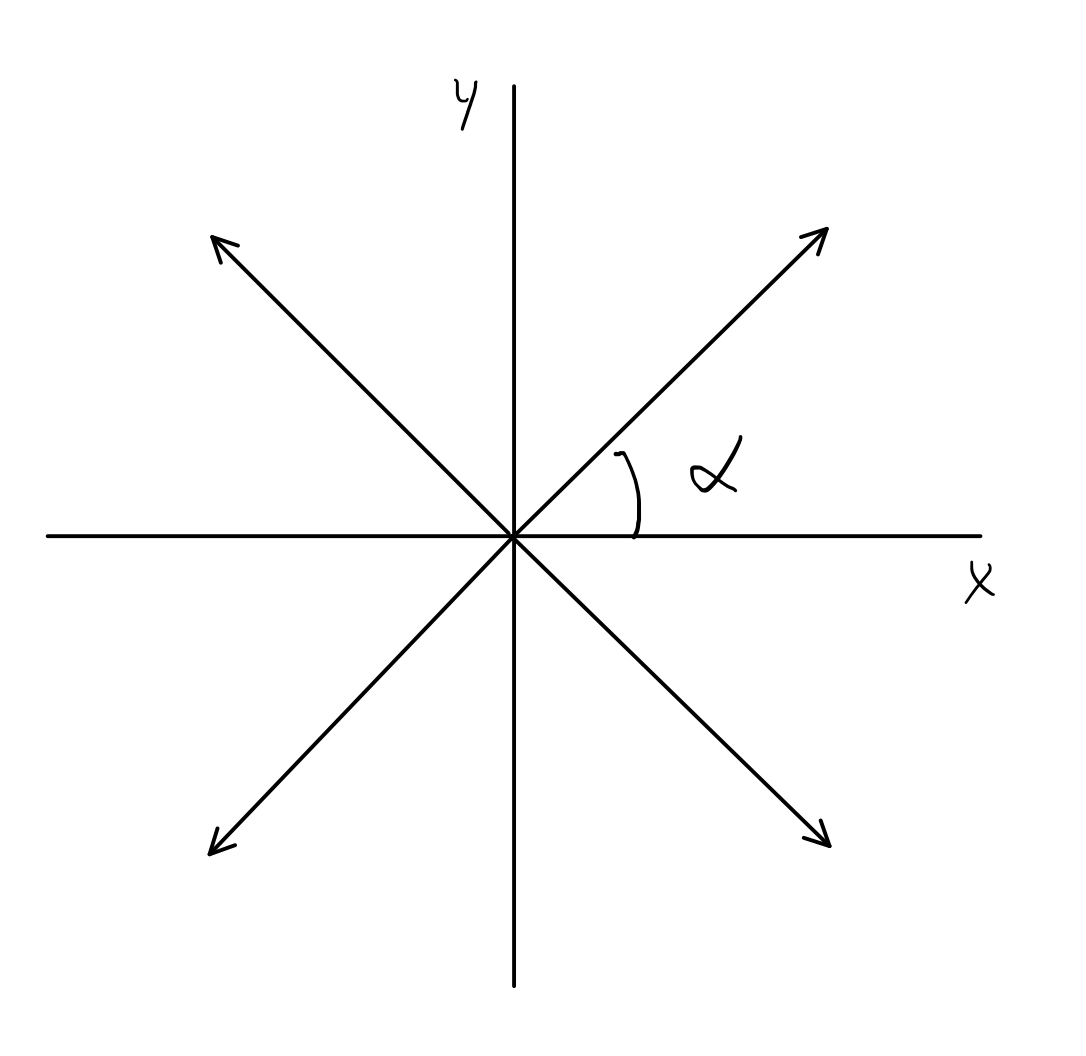
\includegraphics[width=0.4\textwidth]{figures/problem9.png}
    \label{fig:my_label}
\end{figure}

To maximize the uncertainty with respect to $\beta$, 
\begin{align*}
    \frac{\partial}{\partial \beta} \left\langle\left(\Delta S_{x}\right)^{2}\right\rangle\left\langle\left(\Delta S_{y}\right)^{2}\right\rangle &= 0\\
     \frac{\partial}{\partial \beta} \left(\cos ^{2} \beta+\frac{1}{4} \sin ^{4} \beta \sin ^{2} 2  \alpha\right) &= 0\\
     \sin ^2(2 \alpha ) \sin ^3(\beta ) \cos (\beta )-2 \sin (\beta ) \cos (\beta ) &= 0\\
     \sin (\beta ) \cos (\beta ) \left(\sin ^2(2 \alpha ) \sin ^2(\beta )-2\right)&=0\\
     \implies \beta &= 0, \pi\\
\end{align*}
 The maximal uncertainty product is when $\beta = 0,\pi$, which makes implies the maximal $\left\langle\left(\Delta S_{x}\right)^{2}\right\rangle\left\langle\left(\Delta S_{y}\right)^{2}\right\rangle$ is for the pure state $\ket{0}$ or $e^{i \alpha}\ket{1}$. When $\beta \neq 0,\pi$, the product is maximized when $\alpha = \frac{\pi}{4},\frac{3\pi}{4},\frac{-3\pi}{4},\frac{-\pi}{4}$


\newpage

\section{SN 1.23} 
\textit{Consider a three-dimensional ket space. If a certain set of orthonormal kets-say, $\ket{1},\ket{2},$ and $\ket{3}$ - are used as the base kets, the operators $A$ and $B$ are represented by
$$
A \doteq\left(\begin{array}{ccc}
a & 0 & 0 \\
0 & -a & 0 \\
0 & 0 & -a
\end{array}\right), \quad B \doteq\left(\begin{array}{ccc}
b & 0 & 0 \\
0 & 0 & -i b \\
0 & i b & 0
\end{array}\right)
$$ with $a$ and $b$ both real.}

\subsection{}
\textit{Obviously $A$ exhibits a degenerate spectrum. Does $B$ also exhibit a degenerate spectrum?}

\begin{align*}
    \mathrm{det}(B - \lambda) &= 0\\
    b^2 \lambda -b^3+b \lambda ^2-\lambda ^3&= 0\\
\end{align*}
The solutions to the equation $b^2 \lambda -b^3+b \lambda ^2-\lambda ^3= 0$ are $\lambda = -b, b, b$. \newline 
$\therefore$ B is degenerate. 

\subsection{}
\textit{Show that $A$ and $B$ commute.}

\begin{align*}
    AB &= \left(\begin{array}{ccc}
    a & 0 & 0 \\
    0 & -a & 0 \\
    0 & 0 & -a
    \end{array}\right)\left(\begin{array}{ccc}
    b & 0 & 0 \\
    0 & 0 & -i b \\
    0 & i b & 0
    \end{array}\right) \\
    &= \left(\begin{array}{ccc}
     a b & 0 & 0 \\
     0 & 0 & i a b \\
     0 & -i a b & 0 \\
    \end{array}\right)\\
    &\\
    &\\
    BA &= \left(\begin{array}{ccc}
    b & 0 & 0 \\
    0 & 0 & -i b \\
    0 & i b & 0
    \end{array}\right)\left(\begin{array}{ccc}
    a & 0 & 0 \\
    0 & -a & 0 \\
    0 & 0 & -a
    \end{array}\right) \\
    &= \left(\begin{array}{ccc}
     a b & 0 & 0 \\
     0 & 0 & i a b \\
     0 & -i a b & 0 \\
    \end{array}\right)\\
\end{align*}

$$ AB - BA = \left(\begin{array}{ccc}
     a b & 0 & 0 \\
     0 & 0 & i a b \\
     0 & -i a b & 0 \\
    \end{array}\right) - \left(\begin{array}{ccc}
     a b & 0 & 0 \\
     0 & 0 & i a b \\
     0 & -i a b & 0 \\
    \end{array}\right)  = 0$$

\subsection{}
\textit{Find a new set of orthonormal kets that are simultaneous eigenkets of both $A$ and $B .$ Specify the eigenvalues of $A$ and $B$ for each of the three eigenkets. Does your specification of eigenvalues completely characterize each eigenket?}

Starting with the ket $\ket{1}$, with eigenvalue b, the orthonormal eigenkets of $B$ are $\ket{1}, \frac{1}{\sqrt{2}} (i \ket{2} + \ket{3})$, and $\frac{1}{\sqrt{2}} (-i \ket{2} + \ket{3})$. These are simultaneously orthonormal eigenkets of A. 

\newpage
\section{SN 1.26}
\textit{Construct the transformation matrix that connects the $S_{z}$ diagonal basis to the $S_{x}$ diagonal basis. Show that your result is consistent with the general relation
$$
U=\sum_{r}\left|b^{(r)}\right\rangle\left\langle a^{(r)}\right|
$$}

\begin{align*}
\ket{0_x} & = \frac{1}{\sqrt{2}}(\ket{0_z} + \ket{1_z})\\
\ket{1_x} & = \frac{1}{\sqrt{2}}(\ket{0_z} - \ket{1_z})\\
\end{align*}

$$ U = \frac{1}{\sqrt{2}} \left(\begin{array}{cc}
1 & 1 \\
1 & -1
\end{array}\right)$$


$$ U =  \frac{1}{\sqrt{2}}\ketbra{0_x}{0_z} + \frac{1}{\sqrt{2}}\ketbra{1_x}{1_z}$$

This result is consistent with $U=\sum_{r}\left|b^{(r)}\right\rangle\left\langle a^{(r)}\right|$ with $a$ as the $S_z$ basis, and $b$ as the $S_x$ basis.

\end{document}
